\documentclass[a4paper]{article}
\usepackage[top=1cm, bottom=1cm, inner=1cm, outer=1cm]{geometry}
\usepackage{tikz}
\usetikzlibrary{math}
\usepackage{xcolor}

\begin{document}
	\begin{center}
		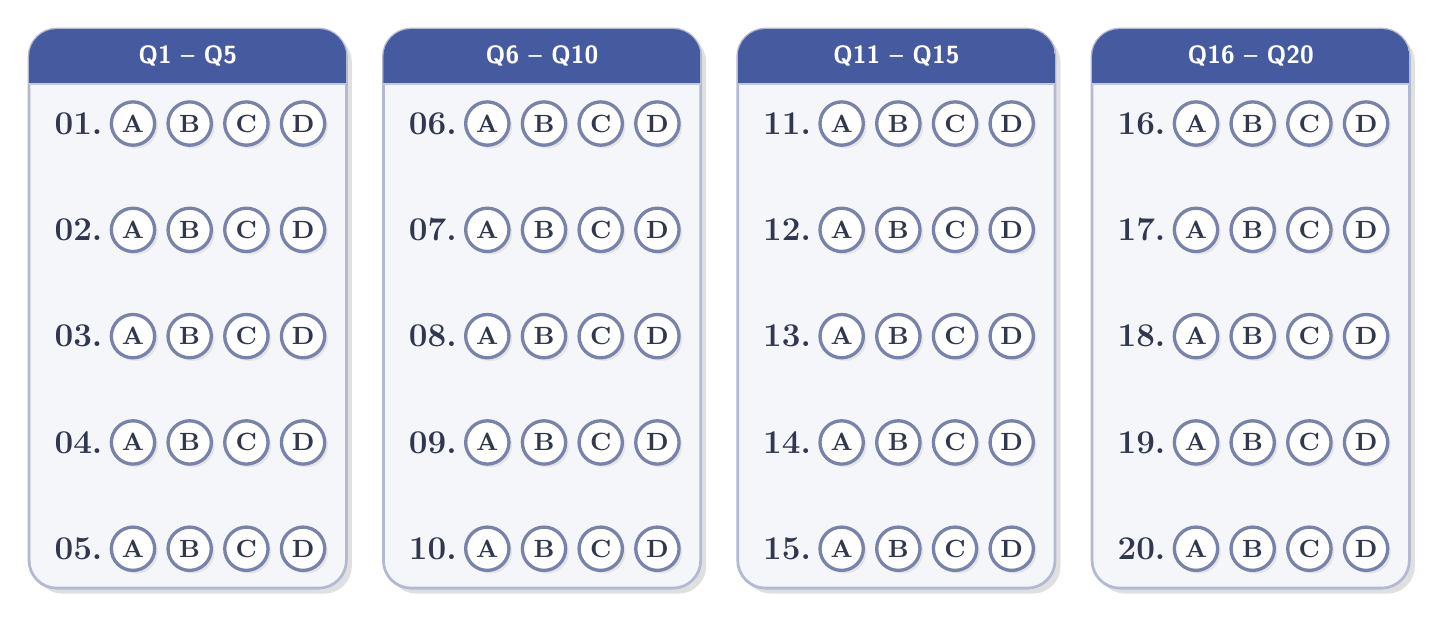
\begin{tikzpicture}
			
			% =============================================================
			%                   USER CONFIGURATION
			%   Edit the values below to customize your answer sheet
			% =============================================================
			
			% --- Question Setup ---
			\def\nquestions{20}        % Total number of questions
			\def\ncols{4}              % Number of columns to split questions into
			\def\options{A,B,C,D}      % Answer options (add/remove letters as needed)
			
			% --- Spacing ---
			\def\numgap{0.4}           % Horizontal gap between question number and first bubble
			\def\bubblegap{0.72}       % Horizontal gap between each bubble
			\def\xsep{4.5}             % Horizontal distance between columns
			\def\ysep{1.35}            % Vertical distance between question rows
			
			% --- Bubble Appearance ---
			\def\circlesize{5.5mm}     % Diameter of each answer bubble
			\def\bubblethick{1.2pt}    % Border thickness of bubbles
			
			% --- Box Appearance ---
			\def\boxpadx{0.2}          % Horizontal padding inside the column box
			\def\boxpady{0.5}          % Vertical padding inside the column box (bottom only)
			\def\boxcorner{10pt}       % Rounded corner radius of the column box
			\def\boxlinewidth{1pt}     % Border thickness of the column box
			
			% --- Header Bar ---
			% Increase freely — question rows will shift down automatically
			\def\headerheight{0.7}     % Height of the colored header bar (in cm, increase as needed)
			\def\headertoppad{0}    % Padding above the header bar (space from box top to header top)
			\def\headerbtmpad{0.5}    % Gap between bottom of header bar and first question row
			
			% --- Colors ---
			\definecolor{boxfill}{RGB}{245,246,250}      % Column box background color
			\definecolor{boxborder}{RGB}{180,185,210}    % Column box border color
			\definecolor{headerfill}{RGB}{70,90,160}     % Header bar background color
			\definecolor{headertext}{RGB}{255,255,255}   % Header text color
			\definecolor{qnumcolor}{RGB}{50,55,80}       % Question number text color
			\definecolor{bubblefill}{RGB}{255,255,255}   % Bubble fill color
			\definecolor{bubbleborder}{RGB}{120,130,170} % Bubble border color
			\definecolor{bubbletext}{RGB}{50,55,80}      % Bubble letter color
			
			% =============================================================
			%   AUTO-COMPUTED VALUES — derived from the settings above
			% =============================================================
			
			\pgfmathsetmacro{\nrows}{ceil(\nquestions/\ncols)}
			\pgfmathtruncatemacro{\nrowsint}{\nrows}
			
			% Total vertical offset from box top to first question row center:
			%   headertoppad  →  header bar  →  headerbtmpad  →  first row
			\pgfmathsetmacro{\firstrowoffset}{\headertoppad + \headerheight + \headerbtmpad}
			
			% =============================================================
			%                   DRAW COLUMN BOXES & HEADERS
			% =============================================================
			
			\foreach \col in {0,...,\numexpr\ncols-1} {
				
				\pgfmathtruncatemacro{\colstart}{\col * \nrowsint}
				\pgfmathtruncatemacro{\colend}{min((\col+1)*\nrowsint, \nquestions)-1}
				\pgfmathtruncatemacro{\nrowsthiscol}{\colend - \colstart + 1}
				\pgfmathtruncatemacro{\qs}{\colstart + 1}
				\pgfmathtruncatemacro{\qe}{\colend + 1}
				
				% Box edges — top is always 0; bottom grows with rows + header + padding
				\pgfmathsetmacro{\bxl}{\col * \xsep - \boxpadx}
				\pgfmathsetmacro{\bxr}{\col * \xsep + \numgap + 4*\bubblegap + \boxpadx + 0.35}
				\pgfmathsetmacro{\byt}{0}   % Box top fixed at y=0
				\pgfmathsetmacro{\byb}{
					-\firstrowoffset                        % space for header
					-(\nrowsthiscol - 1) * \ysep            % space for question rows
					-\boxpady                               % bottom padding
				}
				\pgfmathsetmacro{\bxmid}{(\bxl+\bxr)/2}
				
				% Header bar top/bottom y coordinates (inside box)
				\pgfmathsetmacro{\hbart}{\byt - \headertoppad}              % header bar top
				\pgfmathsetmacro{\hbarb}{\byt - \headertoppad - \headerheight} % header bar bottom
				
				% --- Drop shadow ---
				\draw[
				rounded corners=\boxcorner,
				fill=black!12,
				draw=none
				] (\bxl+0.07, \byt-0.07) rectangle (\bxr+0.07, \byb-0.07);
				
				% --- Main column box ---
				\draw[
				rounded corners=\boxcorner,
				line width=\boxlinewidth,
				draw=boxborder,
				fill=boxfill
				] (\bxl, \byt) rectangle (\bxr, \byb);
				
				% --- Colored header bar (clipped to stay inside rounded box) ---
				\begin{scope}
					\clip[rounded corners=\boxcorner]
					(\bxl, \byt) rectangle (\bxr, \byb);
					\fill[headerfill]
					(\bxl, \hbart) rectangle (\bxr, \hbarb);
				\end{scope}
				
				% --- Thin accent line below header bar ---
				\draw[
				line width=0.6pt,
				draw=boxborder!80
				] (\bxl, \hbarb) -- (\bxr, \hbarb);
				
				% --- Header label centered vertically in the bar ---
				\pgfmathsetmacro{\hbarmid}{(\hbart + \hbarb) / 2}
				\node[
				font=\small\bfseries\sffamily,
				text=headertext,
				anchor=center
				] at (\bxmid, \hbarmid) {Q\qs\ --\ Q\qe};
			}
			
			% =============================================================
			%                   DRAW QUESTIONS & BUBBLES
			% =============================================================
			
			\foreach \i in {0,...,\numexpr\nquestions-1} {
				
				\pgfmathtruncatemacro{\row}{mod(\i, \nrowsint)}
				\pgfmathtruncatemacro{\col}{int(\i / \nrowsint)}
				\pgfmathtruncatemacro{\qnum}{\i + 1}
				
				\pgfmathsetmacro{\x}{\col * \xsep}
				
				% y = 0 (box top) - firstrowoffset (header section) - row * ysep
				% This means row 0 always starts below the header, regardless of header size
				\pgfmathsetmacro{\y}{-\firstrowoffset - \row * \ysep}
				
				% --- Question number ---
				\ifnum\qnum<10
				\node[anchor=west, text=qnumcolor, font=\large\bfseries]
				at (\x, \y) {0\qnum.};
				\else
				\node[anchor=west, text=qnumcolor, font=\large\bfseries]
				at (\x, \y) {\qnum.};
				\fi
				
				% --- Answer bubbles ---
				\foreach \opt [count=\k from 1] in \options {
					\pgfmathsetmacro{\optx}{\x + \numgap + \k * \bubblegap}
					
					% Bubble shadow
					\node[
					circle,
					minimum size=\circlesize,
					inner sep=0pt,
					fill=black!10,
					draw=none
					] at (\optx+0.04, \y-0.04) {};
					
					% Main bubble
					\node[
					draw=bubbleborder,
					circle,
					minimum size=\circlesize,
					inner sep=0pt,
					font=\bfseries\small,
					text=bubbletext,
					fill=bubblefill,
					line width=\bubblethick
					] at (\optx, \y) {\opt};
				}
			}
			
		\end{tikzpicture}
	\end{center}
\end{document}